%نام و نام خانوادگی:
%شماره دانشجویی: 
\مسئله{}
در حوزه متدولوژی‌های \lr{Agile}: \\
الف) چه عواملی باعث می‌شود تا مدل فرآیند توسعه یک نرم‌افزار \lr{Scrum} انتخاب شود یا \lr{Kanban}؟\\
ب) چه تفاوتی بین برد \lr{Scrum} و برد \lr{Kanban} وجود دارد؟

\پاسخ{

الف) از عوامل مهم در انتخاب بین اسکرام (\lr{Scrum}) و کنبن (\lr{Kanban}) می‌توان به موارد زیر اشاره کرد:
\begin{itemize}
\item سابقه تیم در استفاده از مدل چابک:

در مدل اسکرام جلسه‌هایی برای برنامه‌ریزی اسپرینت‌ها (\lr{Sprints}) و بازنگری آنها در ابتدا و انتهای هر اسپرینت برگزار می‌شود. تیم‌هایی که سابقه کار با مدل چابک را ندارند نیاز بیشتری به این جلسات دارند تا بتوانند از یک اسپرینت به اسپرینت بعدی پیشرفت بیشتری داشته باشند. این در حالی‌ است که در تیم‌هایی با سابقه استفاده از چابک، این جلسات باعث هدر رفتن زمان برای تمامی اعضای تیم می‌شود و بنابراین در این شرایط بهتر است از کنبن استفاده شود. 

\item تغییرات احتمالی در طول پروژه:

مدل کنبن برای تطبیق هر چه سریعتر با تغییرات طراحی شده است، به این صورت که به محض وقوع یک تغییر یا ایجاد نیازمندی جدید، تلاش می‌شود در اولین فرصت و در حین کار به موقعیت جدید رسیدگی شود. این در حالی است که در مدل اسکرام محدودیت‌های هر اسپرینت مشخص است و در میانه  مسیر نمی‌توان تغییرات را اعمال کرد، بلکه می‌توان آن‌ها را به اسپرینتهای بعدی منتقل نمود. در صورتی که احتمال تغییر در میانه پروژه کم باشد یا تیم قابلیت تطبیق بالا داشته باشد، استفاده از کنبن توصیه می‌شود. در غیر این صورت اسکرام مدل بهتری خواهد بود. 

\item مدت زمان پروژه:

معمولا اسکرام برای پروژه‌های طولانی‌مدت و بزرگ و کنبن برای پروژه‌های کوتاه مناسب‌ هستند. از آنجایی که در اسکرام تمرکز بر روی تمام کردن اسپرینتها در زمان مشخص است، یک پروژه بزرگ می‌تواند به بخش‌های کوچک‌تری تقسیم شود تا هر یک از بخش ها در اسپرینت مشخصی به پایان برسند. 


\end{itemize}


ب) به یازده تفاوت بین برد‌های کنبن و اسکرام اشاره می‌کنیم:
\begin{itemize}
\item محدودیت تعداد کار‌های در حال انجام

اسکرام کار‌های در حال پیشرفت را در هر چرخه محدود می‌کند و تیم توسعه باید به وظایفی که اول اسپرینت اعلام آمادگی انجامشان را کرده بود متعهد باشد و چیزی نباید جلوی پیشرفت همزمان کارهای مختلف یک اسپرینت را بگیرد.\\
کنبن کارهای در حال انجام را در هر \lr{workflow} محدود می‌کند. مثلا، شماره پنج قسمت صورتی یعنی حداکثر ۵ مورد در ستون در حال انجام می‌تواند باشد.
\end{itemize}

\begin{figure}
	\centering
	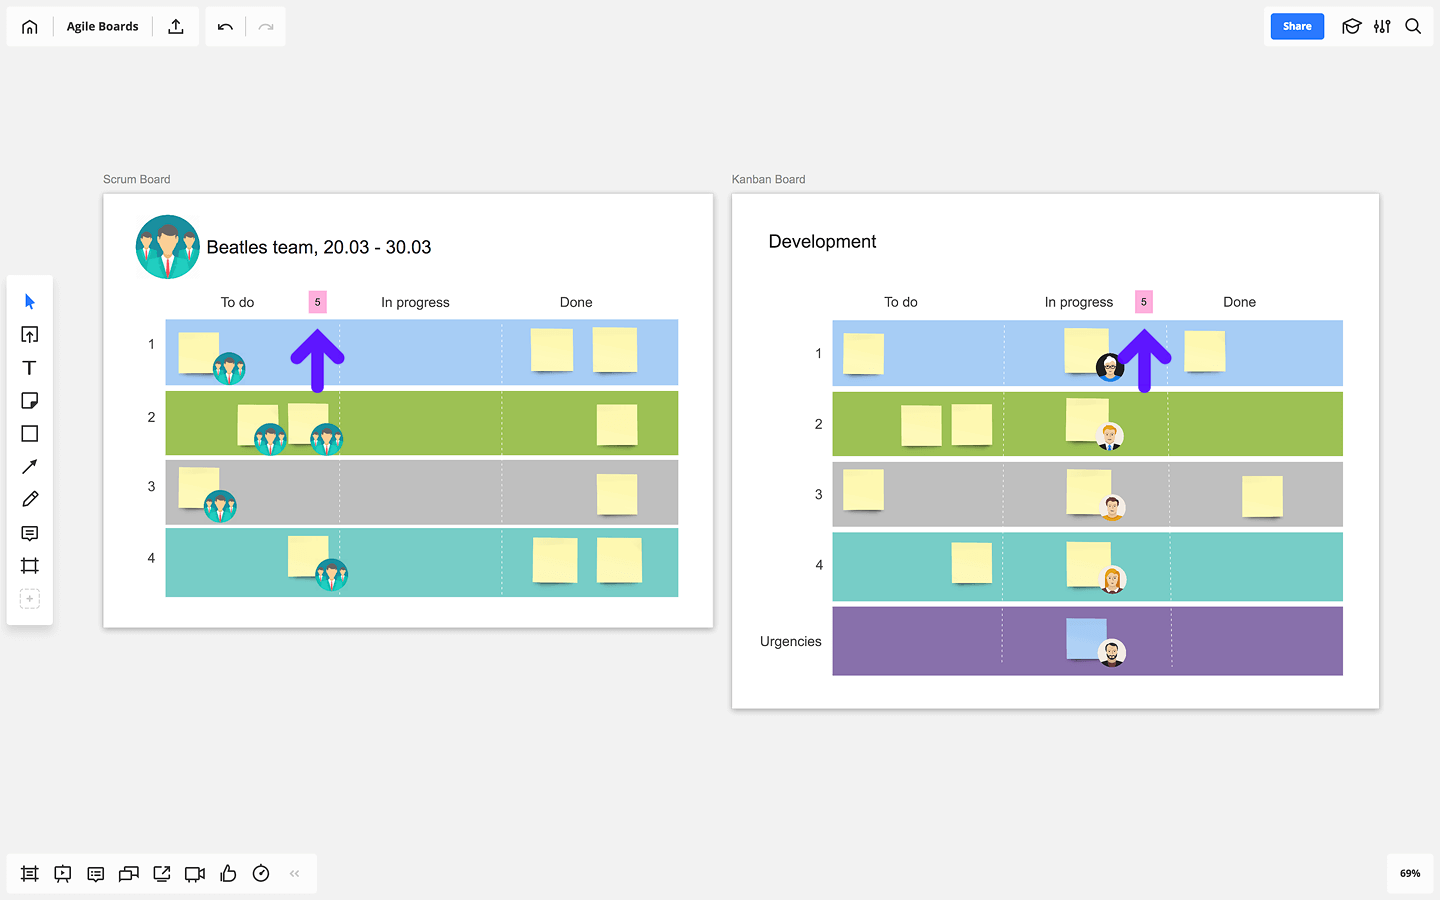
\includegraphics[scale=0.3]{figs/4-2-a}
	\caption{محدودیت تعداد کار‌های در حال انجام}
\end{figure}

\begin{itemize}
\item مالکان

بورد اسکرام متعلق به یک تیم اسکرام است که معمولاً توسط یک رهبر با نام \lr{Srum Master} اداره می‌شود. تیم اسکرام گروهی از افراد است که سابقه‌ی آنان شامل مهارت‌های مورد نیاز برای تکمیل موفقیت‌آمیز همه‌ی وظایف در طول اسپرینت است.
\\
برد کنبن نیازی به یک تیم خاص ندارد و بیشتر به یک گردش کار اختصاص دارد.

\end{itemize}

\begin{figure}
	\centering
	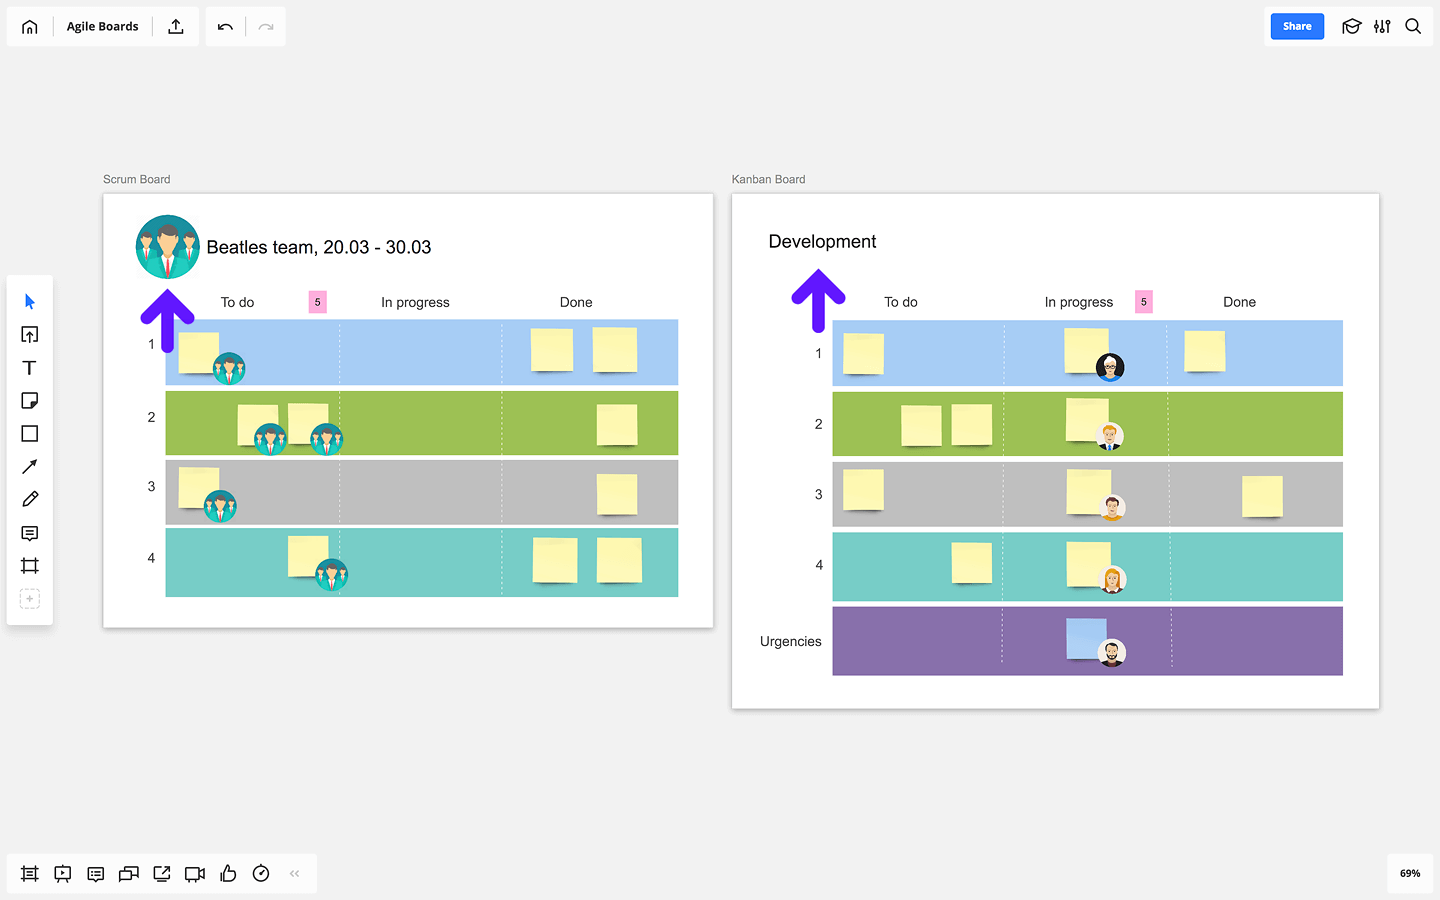
\includegraphics[scale=0.3]{figs/4-2-b}
	\caption{تفاوت مالکیت بین دو برد}
\end{figure}


\begin{itemize}

\item حق وتو برای مالک محصول

اگر تیم به تعدادی از موارد اسپرینت رسیدگی کرده باشد، مالک محصول دیگر نمی‌تواند برد اسکرام را ویرایش کند. اگرچه برد اسکرام برای هر فردی قابل مشاهده است، فقط تیم اسکرام (مالکین برد) می‌توانند آن را ویرایش کنند.
\\
صاحب محصول می‌تواند برد کنبن را ویرایش کند. کنبن درون خود دو "کلاه" را که اعضای تیم می‌توانند بر سر بگذارند تعریف کرده است: \lr{Service Request Manager} و \lr{Service Delivery Manager}. کلاه اول حکم همان مالکیت محصول را دارد.

\item تقسیم وظیفه

در کنبن، یک تیم مسئول تمام وظایف نیست. هر فرد مسئول گام خود در روند کار از کدزنی تا تست و بررسی و ... است. با این حال، کنبن برای رفع تنگنا‌های کاری از تکنیکی به نام \lr{Slack Resource} استفاده می‌کند که به هر منبع غیر گلوگاهی می‌گویند. فرضا اگر عضوی کار خود را انجام داده ولی یک کار پیچیده‌ای در قسمتی از آنالیز کد وجود داشته باشد، می‌تواند انتخاب کند که به تحلیلگر کمک کند یا فعالیت دیگری از صف بردارد.
\item به‌روزرسانی در هر چرخه

تیم اسکرام نباید هیچ مورد جدیدی را در طول اسپرینت به برد اضافه کند. تعداد مواردی که قرار است در یک چرخه‌ی جدید انجام شوند باید در طول جلسه برنامه‌ریزی تنظیم شوند.

هیچ چارچوب زمانی برای به‌روزرسانی یک برد کنبن وجود ندارد و افراد تیم روند را با استفاده از اطلاعات تاریخی قبلی تخمین می‌زنند، زیرا در غیر این صورت فعالیت‌های در حال پیشرفت محدود می‌شوند. به محض اینکه هر کاری از ستون در حال انجام به بخش اتمام منتقل شود، مورد جدیدی اضافه می‌شود.

\item موارد اضطراری

به دلیل داشتن جلسات تحلیلی، برنامه‌ریزی دقیق و اولویت بندی، یک تیم اسکرام به ندرت با موارد غیرمنتظره مواجه می‌شود. درواقع یکی از اهداف اصلی اسکرام تطبیق‌پذیری محصول و پیش‌بینی کردن وضعیت تیم است.

بعضی از تیم‌ها یک بخش اضطراری را به برد کنبن اضافه می‌کنند که به عنوان یک مسیر شنا نشان داده شده است. که در آن قرار است حداکثر سرعت را بدست آورد. مورد اضطراری ممکن است کار فوری پیش‌بینی نشده از بک‌لاگ یا یک کار گلوگاهی روی برد باشد. در این حالت این وضایف برای تیم ارجحیت دارند و برخی از اعضای تیم باید برای انجام سریع‌تر آن اقدام کنند.

\item بک‌لاگ

در تسک‌برد اسکرام، گروه کار‌ها را از بک‌لاگ محصول به بک‌لاگ اسپرینت منتقل می‌کند، که لیستی از چیزهایی است که آنها وظیفه دارند در یک بازه‌ی زمانی مشخص انجام دهند.

اسکرام یوزر استوری را بهترین روش برای تجزیه موارد بزرگ از بک‌لاگ محصول به بک‌لاگ اسپرینت می‌داند. بنابر راهنمای چابک، ویژگی‌ها و وظایف باید همراه با جزئیاتی مانند آزمون‌های پذیرش، طرح‌های رابط کاربری و ... باشند.

کنبن هم از یک روش بک‌لاگ استفاده می‌کند که عموما اما نه الزاما مشابه یک یوزر استوری است.

\item اگر تیم اسکرام به مواردی متعهد شود، برای آن‌ها تخمینی در بازه‌ی اسپرینت می‌زند. اگر کار برای اسپرینت خیلی بزرگ است، به قسمت‌های کوچک‌تر تجزیه می‌شود تا هر مرحله با بازه‌های زمانی اسپرینت مطابقت داشته باشد.

با وجود انتقال وظایف از بخش بک‌لاگ به To-Do از طریق پروپوزال‌ها و \lr{Commitment Point}، قانون خاصی در مورد حجم کار در کنبن وجود ندارد.

\item اولویت‌بندی

در اسکرام، اولویت‌بندی امری ضروری شامل مرتب‌سازی و اصلاح بک‌لاگ محصول برای اسپرینت فعلی، تعیین اولویت‌ها و برآورد منابع در جلسات روزانه اسکرام است. به‌علاوه مهم است که پیش‌بینی کنید چه چیزی در اسپرینت بعدی اهمیت دارد.
\end{itemize}
    
\begin{figure}
	\centering
	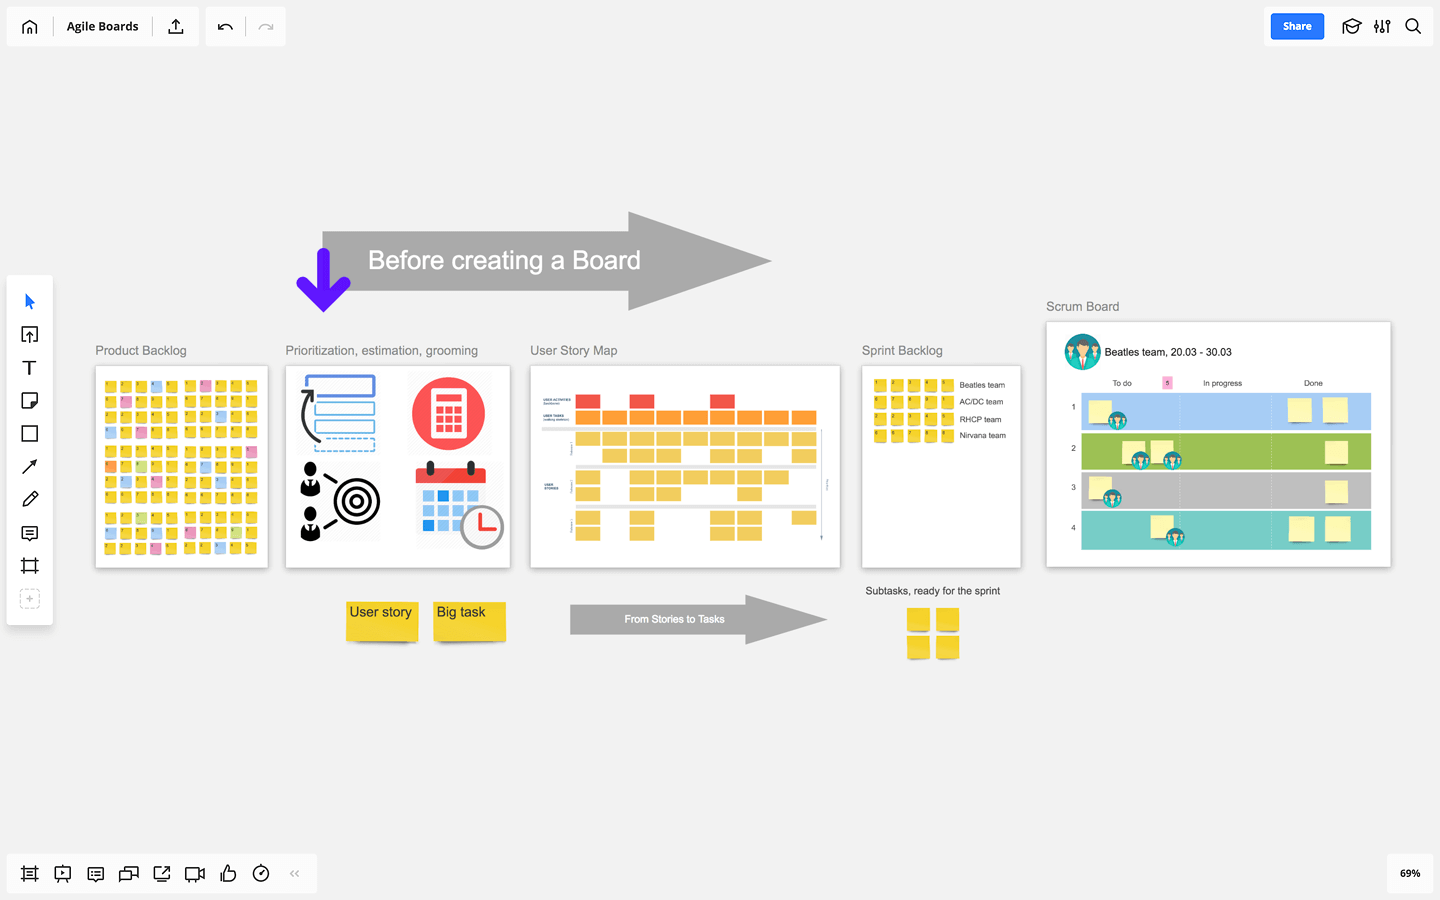
\includegraphics[scale=0.3]{figs/4-2-c}
	\caption{بخش اولویت‌ها در اسکرام}
\end{figure}

کنبن از اولویت‌بندی و برآورد استفاده نمی‌کند، اما برنامه‌ریزی پروژه را با استفاده از پیش‌بینی احتمالی جلو می‌برد.

\begin{figure}
	\centering
	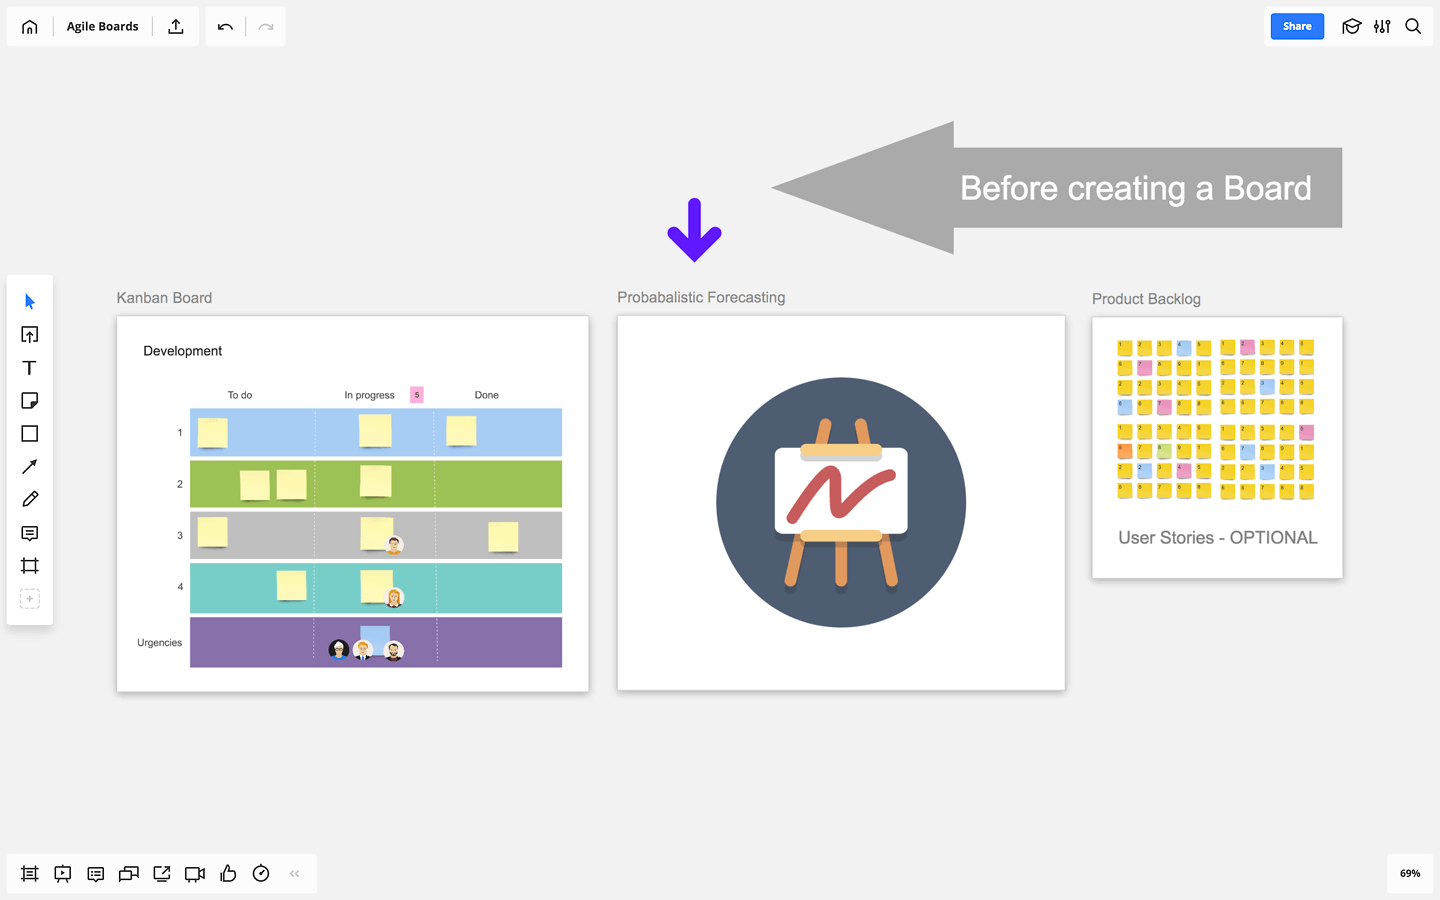
\includegraphics[scale=0.3]{figs/4-2-d}
	\caption{کنبن بخش اولویت‌بندی ندارد}
\end{figure}

\begin{itemize}

\item گزارش‌ها

اسکرام از velocity به عنوان معیار اصلی استفاده می‌کند که با طیف وسیعی از نمودارها و گزارش‌ها مانند
نمودار \lr{Sprint Burndown}، \lr{Sprint Report}، \lr{Epic Burndown}، \lr{Epic Report}، \lr{Release Burndown} و غیره همراه است.

در کنبن نمودارهای خاصی وجود ندارند. اگرچه گزارش‌هایی که در ادامه معرفی می‌کنیم بهتر است به کنبن پین شوند، زیرا معیار اصلی آن \lr{Lead Time} است: نمودار کنترل که زمان چرخه issueها را اندازه‌گیری می‌کند و نمودار جریان تجمعی که وضعیت‌های مختلف کارها را برای یک بازه زمانی خاص نشان می‌دهد.

\item دوره‌های بازنشانی (Reset)

در اسکرام همه استیکرها باید در انتهای هر اسپرینت در قسمت Done باشند، در غیر این صورت اسپرینت ناموفق در نظر گرفته می‌شود. پس از بررسی اسپرینت، تمام برچسب‌ها از برد پاک می‌شوند. فرآیند تنظیم مجدد برد حس خوبی از تکمیل کارهای و بسته‌شدن پرونده‌ی اسپرینت قبلی می‌دهد.

کنبن ابزاری بدون بازه زمانی است، بنابراین نیازی به تنظیم و شروع مجدد نیست. روند کنبن با چرخه عمر پروژه ادامه می‌یابد و موارد جدید و استیکرها در گذر زمان اضافه می‌شوند.

\end{itemize}

}

\subsection*{مراجع}

\begin{latin}
	\begingroup
	\renewcommand{\section}[2]{}%
	
\begin{thebibliography}{9}
%   https://www.student.unsw.edu.au/how-do-i-cite-electronic-sources

	\bibitem{4-1}
	 ‌\textit{Business Adobe}
	Kanban vs Scrum: Which Should You Choose?,  ‌
	accessed at 8 November 2022,
	\url{https://business.adobe.com/blog/basics/kanban-vs-scrum} 

	\bibitem{4-2}
	\textit{Mindtree},
	How to Choose between Kanban and Scrum, 
	acceseed 8 November 2022,
	\url{https://www.mindtree.com/insights/blog/how-choose-between-kanban-and-scrum}

	\bibitem{4-3}
	\textit{Forbes Magazine},
	Kanban vs. Scrum: Which Is Right for You?,
	accessed 8 November 2022,
	\url{https://www.forbes.com/advisor/business/software/kanban-vs-scrum/}
        
	\bibitem{4-4}
	\textit{Guru99},
	Scrum vs Kanban – Difference Between Them,
	accessed 8 November 2022,
	\url{https://www.guru99.com/scrum-vs-kanban.html}

        \bibitem{4-5}
	\textit{Miro},
	Kanban vs Scrum boards,
	accessed 8 November 2022,
	\url{https://miro.com/blog/scrum-kanban-boards-differences/?utm_source=google&utm_medium=cpc&utm_campaign=S|GOO|NB|DE|EN-EN|Pareto-DSA&utm_adgroup=&utm_custom=16426095804&utm_content=585099772766&utm_term=&matchtype=&device=c&location=2276&gclid=CjwKCAiAvK2bBhB8EiwAZUbP1IRGubbogclPbIL1VYJzsHAklKXUaRZ8fe1TP8vYrl_DgUpKr1L3qBoCsiMQAvD_BwE}
        
	
\end{thebibliography}
\endgroup
\end{latin}






